\section{Performance}

The performance of the CLAS12 simulations is measured by comparing the predicted background rates from beam interactions
in the target with the actual experimental rates. The benchmarks are also quantified for each detector geometry and digitization routine.

\subsection{Comparison of Rates with Data}
On December 17, 2017, the nominal luminosity of \cLuminosity
(75 nA on a 5-cm long liquid-hydrogen target) was achieved in CLAS12 for the first time.
The rates in each of the CLAS12 detectors were measured.

The drift chamber hit occupancy was compared for both the FTOn and FTOff configurations. The integrated occupancy
in regions 1, 2, and 3 are summarized in Tables \ref{tab:ftOnComparison} and \ref{tab:ftOffComparison}. The
DC readout time windows of the experiment at the time were different than what was in the simulation, so the data has been scaled
accordingly. The predicted rates agree quite well with the measured ones.

\begin{table}[h]
	\begin{center}
		\begin{tabular}{| c | c | c |}
			\hline \hline
			Region & Data (rescaled) &  GEMC \\
			\hline
			1 &  $2.8\%$  & $2.7\%$ \\
			2 &  $0.6\%$  & $0.8\%$ \\
			3 &  $1.5\%$  & $1.2\%$ \\
		\hline \hline
		\end{tabular}
	\end{center}
	\caption{Drift chamber hit occupancy comparison between simulation and data for the FTOn configuration at full luminosity.}\label{tab:ftOnComparison}
\end{table}

\begin{table}[h]
	\begin{center}
		\begin{tabular}{| c | c | c |}
			\hline \hline
			Region & Data (rescaled) &  GEMC \\
			\hline
			1 &  $1.7\%$  & $1.1\%$ \\
			2 &  $0.3\%$  & $0.4\%$ \\
			3 &  $0.9\%$  & $0.7\%$ \\
		\hline \hline
		\end{tabular}
	\end{center}
	\caption{Drift chambers hit occupancy comparison between simulation and data for the FTOff configuration at full luminosity.}\label{tab:ftOffComparison}
\end{table}


%\begin{figure}
%	\centering
%	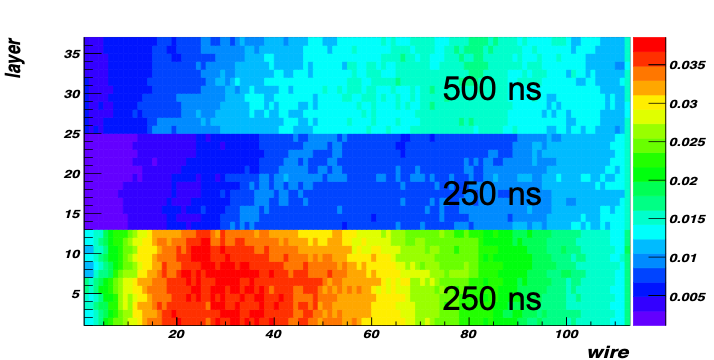
\includegraphics[width=0.99\columnwidth,keepaspectratio]{img/ftOnGemcDCRates.png}
%	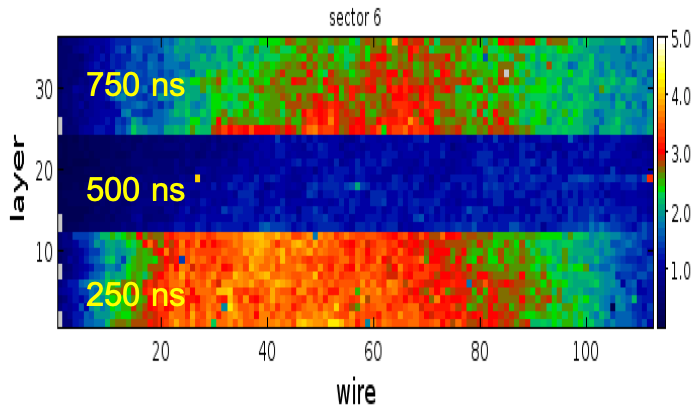
\includegraphics[width=0.99\columnwidth,keepaspectratio]{img/ftOnDataDCRates.png}
%	\caption{Distribution of background events in the Drift Chamber region 1 for the FT On configuration.
%             Top: GEMC. Bottom: data.}
%	\label{fig:ftOnComparison}
%\end{figure}


%\begin{figure}
%	\centering
%	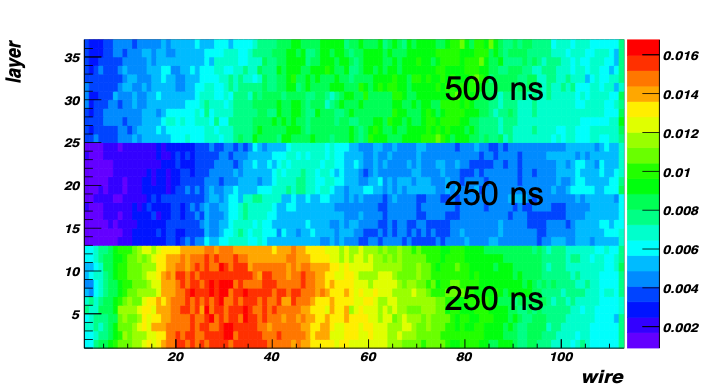
\includegraphics[width=0.99\columnwidth,keepaspectratio]{img/ftOffGemcDCRates.png}
%	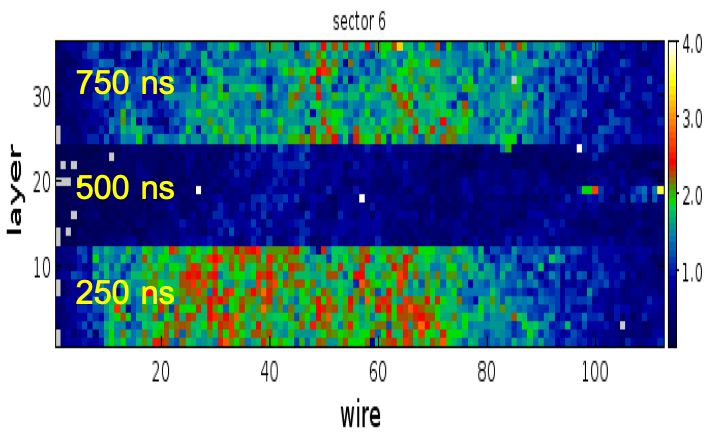
\includegraphics[width=0.99\columnwidth,keepaspectratio]{img/ftOffDataDCRates.png}
%	\caption{Distribution of background events in the Drift Chamber region 1 for the FT Off configuration.
%             Top: GEMC. Bottom: data.}
%	\label{fig:ftOffComparison}
%\end{figure}

Similar agreements were found with the rates in the other CLAS12 detectors. In particular:

\begin{itemize}
	\item FTOF: good agreement with data for the PMT currents \cite{ftof-nim};
	\item CTOF good agreement with data for the upstream PMT counter rates, while the downstream counter rates;
		  are about a factor of three lower, probably due to not handling light signals produced in the light guides \cite{ctof-nim};
	\item FT: good agreement with data for PMT currents and radiation doses \cite{ft-nim}.
\end{itemize}


\subsection{Benchmarks}

The GEMC event simulation rate has been measured for single and multiple tracks. The numbers reported here
refer to averages over several 2017 laptops, desktops, and computing farm nodes, and refer to running GEMC in single-threaded mode.
The full CLAS12 geometry has been used, with a Runge-Kutta field integration algorithm
and linear interpolation for both the solenoid and the torus fields.
Single meson tracks in the forward region are simulated with an event rate of about 10 Hz.
Electron rates are about half as fast due to shower simulations in the EC and PCAL calorimeters and
Cherenkov photon production in both the HTCC and the LTCC, for an average of 5 Hz.

A quantitative study of the event rate for 3 particles (2 in the Forward Detector, one in the Central Detector)
details the time spent in each detector geometry and digitization and in each magnetic field.
The particles generated are:

\begin{itemize}
	\item one 7 GeV electron between polar angles 15\mdeg \ and 25\mdeg;
	\item one 2 GeV photon between polar angles 15\mdeg \ and 25\mdeg;
	\item one 2 GeV proton at $\theta=$90\mdeg.
\end{itemize}

The results are shown in Table \ref{tab:benchmarks}. The final rate for the 3 particles in the
complete CLAS12 setup is 1.9 Hz.

\begin{table}[h]
	\begin{center}
		\begin{tabular}{ c | c | c | c }
			 \hline \hline
			 & Rate (Hz) &  ms / event &  $\%$ of total\\
			\hline
Target   &  555.8  &   1.8   & 0.3  \\
SVT      &  365.9  &   0.9   & 0.2  \\
MM       &  48.9   &   17.7  & 3.4  \\
CTOF     &  48.7   &   0.1   & 0.0  \\
Solenoid &  15.8   &   42.8  & 8.1  \\
HTCC     &  11.5   &   24.0  & 4.5  \\
FT       &  11.2   &   2.4   & 0.4  \\
DC       &  8.1    &   33.2  & 6.3  \\
LTCC     &  6.5    &   30.6  & 5.8  \\
FTOF     &  6.1    &   9.6   & 1.8  \\
PCAL     &  2.8    &   196.2 & 37.1 \\
EC       &  2.0    &   134.5 & 25.4 \\
Torus    &  1.9    &   34.7  & 6.6  \\
		\hline \hline
		\end{tabular}
	\end{center}
	\caption{GEMC simulation benchmarks in each CLAS12 detector. The calorimeters are responsible for more than
             half the computing time, due to shower simulations. Swimming in the magnetic fields accounts for about 15$\%$ of the total CPU time.}
\label{tab:benchmarks}
\end{table}

\noindent Simulations that include the complete beam-target interactions using the full nominal luminosity
of \cLuminosity are made using 124,000 electrons per event. In this case the time to complete one event varies
between one and two minutes depending on the CPU type and available memory.

































